\chapter{Olhó-passarinho: Aplicação Web}\label{chap:chap4}

Neste capítulo será abordada a ferramenta desenvolvida com a descrição da arquitetura implementada, do processamento da informação de espaço e tempo e da sua integração com a informação visual de modo a aplicar a tarefa de \textit{clustering}. Por fim será apresentada a visualização dos resultados ilustrativos.

\section{Arquitetura do Sistema}

A arquitetura do sistema desenvolvido é apresentada na Figura~\ref{fig:archsys}. Esta apresenta uma divisão entre os serviços externos e o modelo desenvolvido. Este modelo foi desenhado de modo a que existisse uma separação entre o tratamento de toda a parte de processamento dos dados e a visualização. Assim existi um \textit{back-end} com todos os ficheiros e módulos desenvolvidos e um \textit{front-end} que representa a aplicação web para visualização dos resultados. No \textit{back-end} existe também uma divisão entre dois módulos fundamentais, o módulo de processamento da informação visual, responsável por tratar a informação das imagens como descrito no Capítulo~\ref{chap:chap3}, e o módulo que utiliza essa informação através do processo de \textit{Data Mining} já desenvolvido no TweeProfiles~\cite{Cunha2013}.

%de modo a que essa informação possa ser utilizada pelo módulo responsável pelo processo de \textit{Data Mining} já desenvolvido no TweeProfiles~\cite{Cunha2013}. 

Os serviços externos correspondem à base de dados MongoDB para a recolha dos tweets e os serviços Twitter e Instagram para a recolha das imagens através do URL. No caso do modelo desenvolvido, o \textit{back-end} guarda os ficheiros JSON com os dados e as imagens necessárias, tanto para o módulo de processamento da informação visual como para a extração e processamento do dados espaço-temporais, explicados na Secção~\ref{sec:infoesptmp}. Os dados processados no módulo da informação visual e os dados espaço-temporal extraídos dos tweets são assim utilizados no processo de \textit{Data Mining}, onde é aplicada a tarefa de \textit{clustering} como explicado na secção~\ref{sec:finalclustering} apresentada mais adiante. Deste processo resultam os \textit{clusters} calculados através de vários parâmetros, sendo esta informação armazenada em ficheiros. Por fim, foi utilizada a \textit{microframework} Flask~\cite{flask} para desenvolvimento de aplicações web em Python, que permitiu o desenvolvimento da aplicação Olhó-passarinho para visualização dos resultados. 

\begin{figure}[h]
\centering
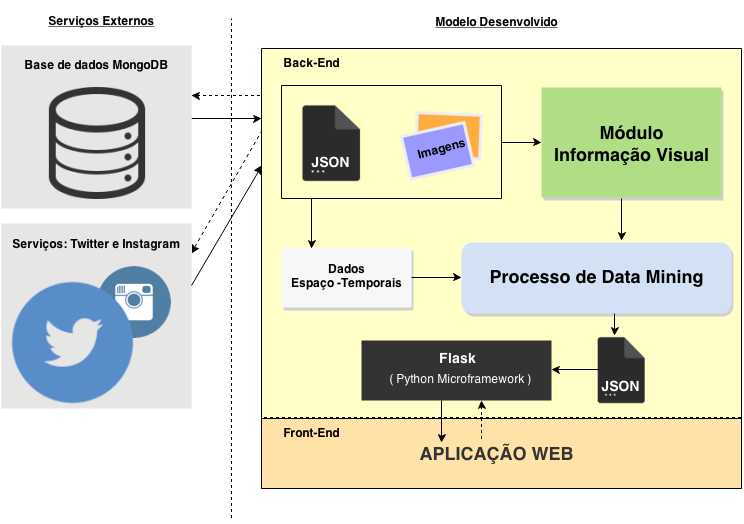
\includegraphics[width=1.0\linewidth]{./figures/arquitetura_sistema}
\caption{Arquitetura do sistema completo}
\label{fig:archsys}
\end{figure}


\section{Informação Espaço-Temporal} \label{sec:infoesptmp}

Uma das características principais tanto do TweeProfiles como do Olhó-passarinho é a combinação das dimensões espaço-temporais com o conteúdo. Para isto ser possível foi realizada a recolha da informação espacial e temporal dos tweets para o cálculo das respetivas matrizes de distância entre tweets. Esta informação apenas foi recolhida dos tweets associados às imagens armazenadas localmente. É importante referir ainda que, tal como exposto na Secção~\ref{sec:matdist}, os dados foram divididos em três subconjuntos com 1988 tweets cada.

Em primeiro lugar foi recolhida a informação espacial. Neste caso os dados possuem a informação de latitude e longitude do ponto onde foi enviado o tweet. É importante lembrar que todos os tweets possuem informação de geolocalização, tendo este sido um dos critérios de seleção dos mesmo como explicado na Secção~\ref{sec:dados}. Para calcular a distância entre tweets utilizou-se a função distância Haversine abordada na Secção~\ref{subsubsec:space}. Neste caso foi calculada a distância em quilómetros, tendo sido considerado o valor do raio da Terra igual a 6371 Km.

Posteriormente foi então recolhida a informação temporal dos tweets, sendo que esta informação contém as três primeiras letras do dia e mês, o número do dia, a hora, minutos e segundo, o fuso horário e o ano da partilha do tweet. Assim o informação temporal apresenta-se como o exemplo ilustrativo seguinte: Tue Jun 18 17:02:09 +0000 2013. Para o cálculo da distância entre datas foi utilizada a função distância Euclidiana, que se pode resumir ao módulo da diferença entre o tempo de dois tweets.

Como resultado, obteve-se para cada dimensão três matrizes de 1988 x 1988. Cada uma dessas três matrizes de cada dimensão representa um subconjunto dos dados e consequentemente um intervalo de tempo. Neste caso cada subconjunto temporalmente é representado na Tabela~\ref{tab:distemp}

\begin{table}[h]
\centering
\begin{tabular}{|c|c|c|c|c|}
\hline
\textbf{}              & Hora de início & Data de início      & Hora de fim & Data de fim         \\ \hline
\textbf{Subconjunto 1} & 13:01:46       & 17 de Junho de 2013 & 03:14:05    & 18 de Junho de 2013 \\ \hline
\textbf{Subconjunto 2} & 03:14:15       & 18 de Junho de 2013 & 00:40:08    & 19 de Junho de 2013 \\ \hline
\textbf{Subconjunto 3} & 00:40:29       & 19 de Junho de 2013 & 23:06:54    & 19 de Junho de 2013 \\ \hline
\end{tabular}
\caption{Distribuição temporal entre os diferentes subconjuntos de dados}
\label{tab:distemp}
\end{table}

%\begin{description}
%\item[Subconjunto 1]
%\item Início: 13:01:46 do dia 17 de Junho de 2013 
%\item Fim: 03:14:05 do dia 18 de Junho de 2013
%
%\item[Subconjunto 2]
%\item Início: 03:14:15 do dia 18 de Junho de 2013 
%\item Fim: 00:40:08 do dia 19 de Junho de 2013
%
%\item[Subconjunto 3]
%\item Início: 00:40:29 do dia 19 de Junho de 2013 
%\item Fim: 23:06:54 do dia 19 de Junho de 2013
%\end{description}

%\textbf{Nota:} Devo colocar mais informação estatística sobre os dados?

\section{Clustering da Informação Visual, Espacial e Temporal} \label{sec:finalclustering}

A tarefa de \textit{clustering} é o último passo para a obtenção dos resultados finais. Este é o processo que engloba os dados resultantes de todo o processamento da informação tratada e discutida anteriormente.

Para a tarefa de \textit{clustering} optou-se pelo mesmo algoritmo utilizado no TweeProfiles~\cite{Cunha2013}, o DBSCAN. Este apresenta algumas vantagens na utilização de dados recolhidos de redes sociais, pois não necessita de uma predefinição do número de \textit{clusters} que se pretende obter, sendo este definido através da distribuição em densidade dos objetos, como referido na Secção~\ref{subsec:dbscan}.

Antes de utilizar os dados para a tarefa de \textit{clustering}, neste caso as matrizes já calculadas com as distâncias entre tweets para as dimensões temporal, espacial e de conteúdo visual, foi necessário realizar a normalização das distâncias através da função normalização mínimo-máximo:

\begin{equation}
x' = \frac{x - x_{min} }{x_{max} - x_{min} }
\label{eq:norm}
\end{equation}
em que $ X_{max} $ é o valor máximo presente na matriz e $ X_{min} $ o valor mínimo. Neste caso o valor mínimo será sempre 0, que equivale à distância de um objeto a si mesmo. Assim a equação simplificada é apresentada na equação~\ref{eq:norm1}

\begin{equation}
x' = \frac{x}{x_{max}}
\label{eq:norm1}
\end{equation}

Após a normalização, realizou-se a combinação entre as matrizes, com atribuição de vários pesos a cada matriz, de forma a que a soma dos diferentes pesos fosse igual a 1. Para isso optou-se por dividir os pesos em fatores de 0.333, em que os valores de cada matriz podem assumir os pesos: 0, 0.333, 0.666, 1.

%A tabela~\ref{tab:pesos} apresenta as diferentes combinações possíveis de pesos para as diferentes dimensões
%
%\begin{table}[h]
%\centering
%\begin{tabular}{|c|c|c|c|}
%\hline
%\textbf{Combinação} & \textbf{Visual} & \textbf{Espacial} & \textbf{Temporal} \\ \hline
%1 & 1.000 & 0.000 & 0.000 \\ \hline
%2 & 0.666 & 0.333 & 0.000 \\ \hline
%3 & 0.666 & 0.000 & 0.333 \\ \hline
%4 & 0.333 & 0.333 & 0.333 \\ \hline
%5 & 0.000 & 1.000 & 0.000 \\ \hline
%6 & 0.333 & 0.666 & 0.000 \\ \hline
%7 & 0.000 & 0.666 & 0.333 \\ \hline
%8 & 0.000 & 0.000 & 1.000 \\ \hline
%9 & 0.333 & 0.000 & 0.666 \\ \hline
%10 & 0.000 & 0.333 & 0.666 \\ \hline
%\end{tabular}
%\vspace{2 mm}
%\caption{Tabela com as possiveis distribuições de pesos entre as várias dimensões}
%\label{tab:pesos}
%\end{table}

\section{Visualização} \label{sec:visu}

A aplicação web desenvolvida é responsável pela visualização dos resultados obtidos pela tarefa de \textit{clustering}. Esta apresenta três secções principais de visualização dos \textit{clusters} pelas diferentes dimensões utilizadas. O primeiro é um mapa, onde é apresentada a distribuição dos tweets, como pode ser visto na Figura~\ref{fig:map1} e a respetiva distribuição dos \textit{clusters} geograficamente. Este foi desenvolvido recorrendo à API Javascript do Google Maps v3~\cite{googlemapsapi} disponibilizada pela Google, sendo toda ela controlada através da linguagem de programação Javascript. É possível utilizar e controlar um mapa de modo a adicionar diferentes componentes visuais. Os tweets foram assim representados por pequenos círculos azuis, e os \textit{clusters} por círculos vermelhos com transparência como será ilustrado mais à frente. 

\begin{figure}[h]
\centering
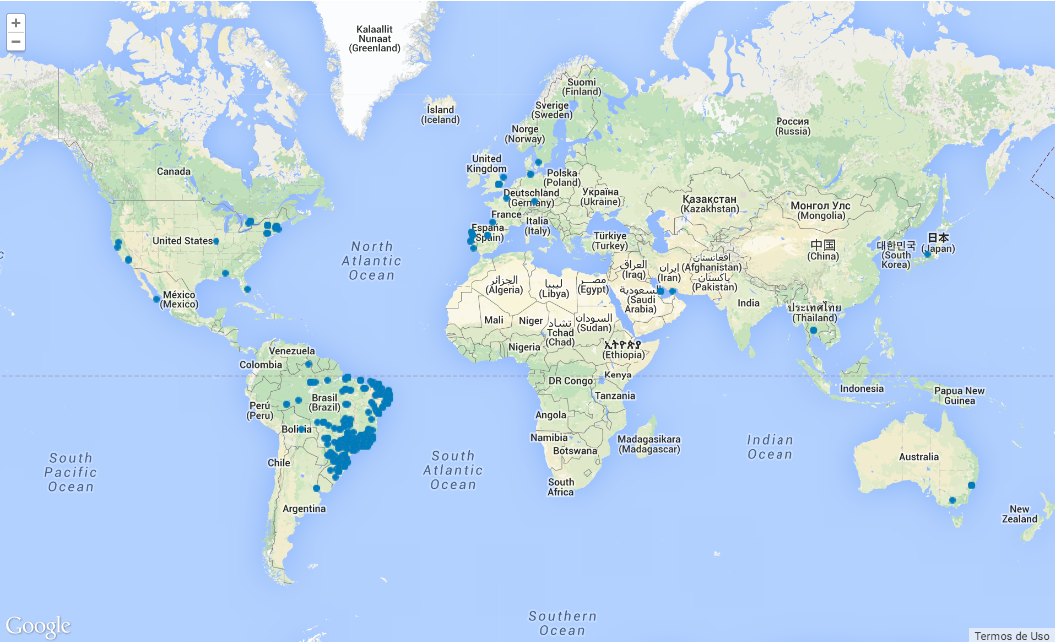
\includegraphics[width=1.0\linewidth]{./figures/olhopassarinho/map1.png}
\caption{Distribuição de tweets na dimensão espacial}
\label{fig:map1}
\end{figure}

A segunda secção é responsável pela representação da distribuição dos \textit{clusters} na dimensão temporal e para isso foi utilizada a ferramenta Google Charts, mais especificamente a API Timeline~\cite{googletimeline}. Esta, tal como a API do Google Maps, também é desenvolvida em Javascript, e permite criar um gráfico com barras de duração temporal, como podemos ver na figura~\ref{fig:timeex}. 

\begin{figure}[h]
\centering
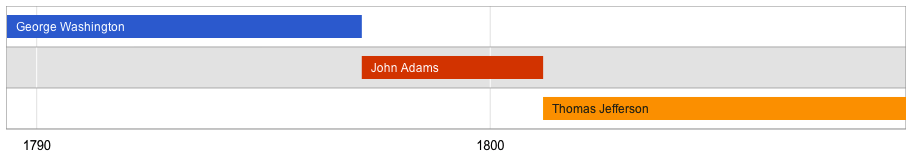
\includegraphics[width=1.0\linewidth]{./figures/olhopassarinho/time_example.png}
\caption{Exemplo ilustrativo da ferramenta Timeline. \textit{Retirada de}~\cite{googletimeline}}
\label{fig:timeex}
\end{figure}

Por último, a secção de visualização de imagens que pertencem a um \textit{cluster}, onde é apresentada uma matriz com nove imagens, como apresentado na Figura~\ref{fig:mat99}. As imagens presentes nos \textit{clusters} são escolhidas aleatoriamente, havendo ainda a possibilidade de ir modificando as imagens visíveis. É possível também clicar numa das imagens, visualizar a mesma em tamanho maior, ver a informação relativa ao tweet a que a imagem pertence, o nome do utilizador, o texto e a data de partilha do tweet. Para além disto, é possível aceder ao tweet original através de um botão com essa indicação. Esta secção apresenta ainda o nome e a informação temporal do \textit{cluster}.

\begin{figure}[h]
\centering
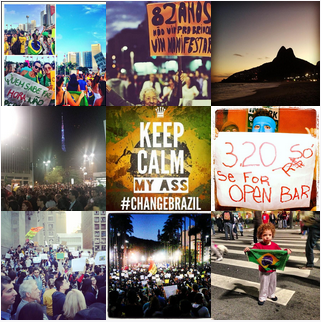
\includegraphics[width=0.4\linewidth]{./figures/olhopassarinho/mat99.png}
\caption{Exemplo ilustrativo da visualização da matriz para visualização de nove imagens.}
\label{fig:mat99}
\end{figure}


A aplicação apresenta também os controlos para escolher o subconjunto que se pretende visualizar, e controlos para definir o peso que se pretende atribuir a cada dimensão.

\section{Resultados Ilustrativos}

Nesta secção serão apresentados alguns resultados ilustrativos do tipo de conhecimento que se pode obter com a ferramenta Olhó-passarinho. Neste relatório não é possível apresentar todos os resultados devido ao número de diferentes combinações possíveis. 

A dimensão dos círculos que representam os \textit{clusters} é proporcional ao número de tweets presentes nesse mesmo \textit{clusters}, isto é, quanto maior o número de tweets maior é a respetiva circunferência. Assim a Figura~\ref{fig:map31} um exemplo da visualização da distribuição dos \textit{clusters} no espaço geográfico onde é atribuída 100\% do peso a dimensão espacial. Podemos ver que foram gerados sete \textit{clusters} e que existe uma clara divisão espacial entre eles. Podemos localizar um \textit{cluster} na Europa mais sobre a zona do Reino Unido, dois na Ásia em que um situa-se sobre países junto do Golfo do Pérsico e outro sobre o Japão, um na Austrália, dois na América do Norte mais especificamente sobre o Oeste e o Este dos Estados Unidos da América e por último na América do Sul, sendo o \textit{cluster} de com maior dimensão relativamente aos outros, e localiza-se sobre o Brasil.

\begin{figure}
\centering
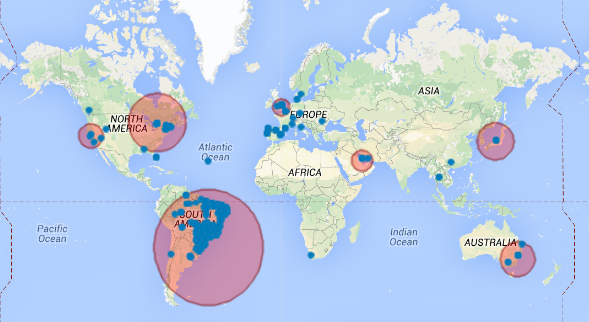
\includegraphics[width=0.8\linewidth]{./figures/olhopassarinho/map31}
\caption{Distribuição dos \textit{clusters} no mapa calculado exclusivamente através da dimensão espacial}
\label{fig:map31}
\end{figure}

Já no caso em que é atribuído 100\% do peso apenas à dimensão temporal obtemos dois \textit{cluster} como percetível pela Figura~\ref{fig:map32}. No caso da sua visualização temporal, verificamos pela Figura~\ref{fig:time11} que obtêm-se um intervalo temporal em que não existe nenhum tweet associado a um \textit{cluster}, podendo-se dever ao facto de aquele período apresentar um volume muito mais reduzido de tweets levando a um dispersão dos mesmo no tempo e consequentemente a uma menor densidade de tweets.
%apenas um \textit{cluster} como percetível pela Figura~\ref{fig:map32}. Este \textit{cluster} encontra-se sobre o Brasil, devido a densidade de tweets. A obtenção de apenas um \textit{cluster} deve-se ao fato de os tweets se encontrem na sua maioria em intervalos de tempo muito curtos e num espaço de tempo por sí só muito reduzido, como podemos ver na Figura~\ref{fig:time11}, em que temos um duração de menos de 24 horas.

\begin{figure}[!h]
\centering
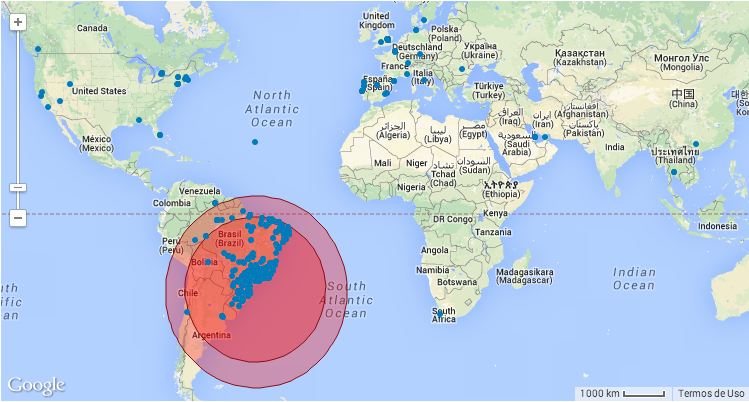
\includegraphics[width=0.9\linewidth]{./figures/olhopassarinho/map32}
\caption{Projeção do \textit{Clusters} no mapa calculado exclusivamente através da dimensão temporal}
\label{fig:map32}
\end{figure}

\begin{figure}[!h]
\centering
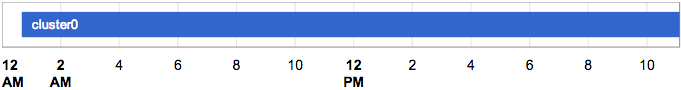
\includegraphics[width=0.9\linewidth]{./figures/olhopassarinho/time11}
\caption{Projeção do \textit{Clusters} no tempo calculado exclusivamente através da dimensão temporal}
\label{fig:time11}
\end{figure}

Para o caso da atribuição de 100\% do peso apenas ao conteúdo visual, o resultado ilustrativo no mapa é apresentado na Figura~\ref{fig:map33}. Para este caso temos a representação de 3 \textit{clusters}. Estes estão localizados sobre o Brasil e apresentam tamanhos distintos, proporcionais ao número de tweets.

\begin{figure}[!h]
\centering
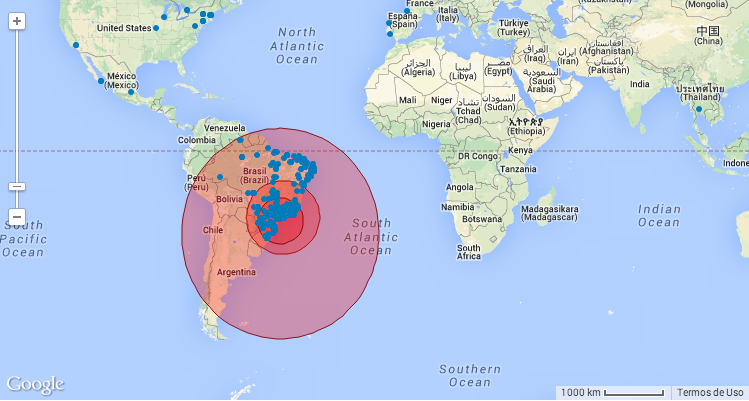
\includegraphics[width=0.8\linewidth]{./figures/olhopassarinho/map33}
\caption{Projeção do \textit{Clusters} no mapa calculado exclusivamente através do conteúdo visual}
\label{fig:map33}
\end{figure}

Como referido na Secção~\ref{sec:visu}, o Olhó-passarinho permite a visualização do conteúdo visual dos \textit{clusters}. A Figura~\ref{subfig:im01} apresenta a visualização de uma amostra de imagens pertencentes a um \textit{cluster}. Neste caso o \textit{cluster} é o mais pequeno representado na Figura~\ref{fig:map33} e contém apenas 9 imagens, o número mínimo definido para a criação de um \textit{cluster}. É visível que estas apresentam o mesmo conteúdo visual, uma bandeira do Brasil e uma citação de uma pessoa com o nome de Federico Devito. Este pormenor pode ser visualizado nas Figuras~\ref{subfig:im02} e \ref{subfig:im02}

\begin{figure}[h]
\centering
	\begin{subfigure}[b]{0.32\textwidth}
	\centering
	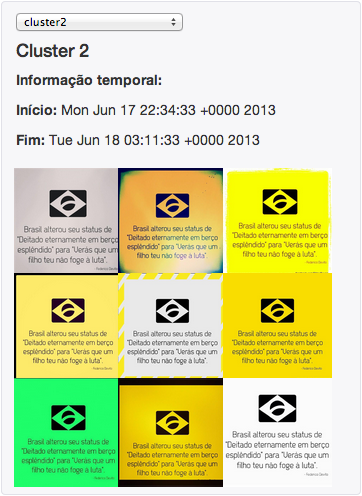
\includegraphics[width=0.95\linewidth]{./figures/olhopassarinho/c2_ex1_im100_1718}
	\caption{Visualização de uma amostra de imagens do um \textit{cluster} }
	\label{subfig:im01}
	\end{subfigure}
	~
	\begin{subfigure}[b]{0.32\textwidth}
	\centering
	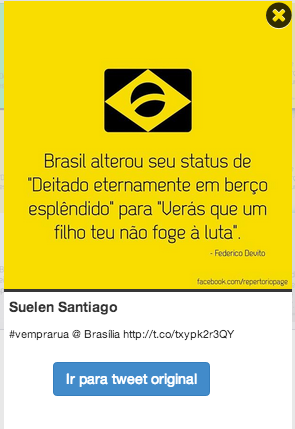
\includegraphics[width=0.9\linewidth]{./figures/olhopassarinho/c2_ex2_im100_1718}
	\caption{ Visualização de uma das imagens do \textit{cluster} }
	\label{subfig:im02}
	\end{subfigure}
	~
	\begin{subfigure}[b]{0.32\textwidth}
	\centering
	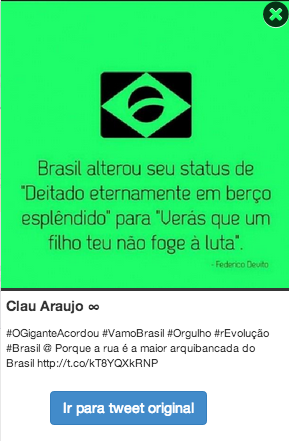
\includegraphics[width=0.85\linewidth]{./figures/olhopassarinho/c2_ex3_im100_1718}
	\caption{ Visualização de outra imagem do \textit{cluster} }
	\label{subfig:im03}
	\end{subfigure}
\caption{Exemplo da visualização do conteúdo visual de um \textit{cluster} calculado com 100\% do peso para a dimensão das imagens}
\label{fig:im00}
\end{figure}

% ------

O exemplo apresentado em seguida mostra-nos o resultado da combinação entre dimensões com atribuição do mesmo peso a cada uma delas. Assim cada dimensão presenta um peso de 33.33\%. A Figura~\ref{fig:map4} ilustra a distribuição dos \textit{clusters} no espaço. Por outro lado, a Figura~\ref{fig:temp4} mostra a distribuição dos mesmo \textit{clusters}, mas neste caso, na dimensão temporal.
\vspace{2mm}

\begin{figure}[!h]
\centering
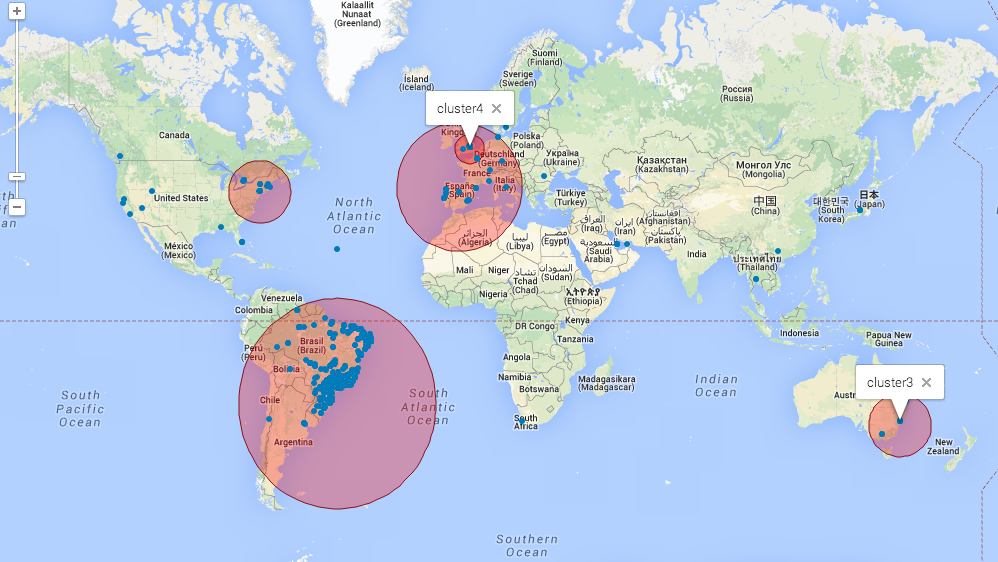
\includegraphics[width=1\linewidth]{./figures/olhopassarinho/map_ex1_im33_e33_t33_1819}
\caption{Projeção dos \textit{Clusters} no mapa com peso atribuído a cada dimensão de 33.33\%}
\label{fig:map4}
\end{figure}

\begin{figure}[h]
\centering
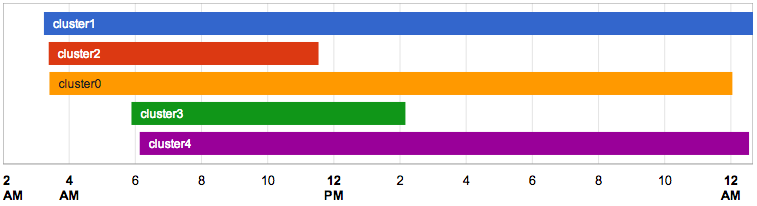
\includegraphics[width=1\linewidth]{./figures/olhopassarinho/temp_ex1_im33_e33_t33_1819}
\caption{Projeção dos \textit{Clusters} no tempo com peso atribuído a cada dimensão de 33.33\%}
\label{fig:temp4}
\end{figure}

No mapa podemos ver a identificação do \textit{Cluster} 3 localizado na Austrália e o \textit{Cluster} 4 no Reino Unido. Uma amostra do seu conteúdo pode ser visualizado na Figura~\ref{fig:im40}. Aqui podemos notar que o conteúdo visual em ambos os \textit{clusters} são muito semelhantes, sendo assim percetível neste caso a influência das dimensões espaço-temporal. 

\begin{figure}[t!]
\centering
	\begin{subfigure}[b]{0.45\textwidth}
	\centering
	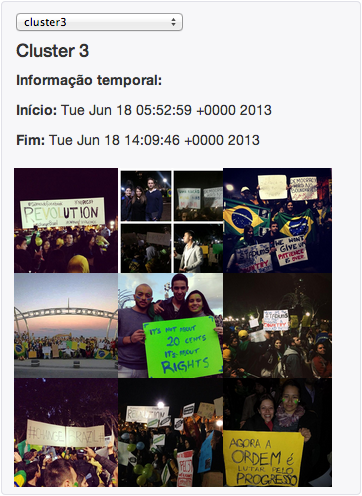
\includegraphics[width=0.9\linewidth]{./figures/olhopassarinho/c3_ex1_im33_e33_t33_1819}
	\caption{Visualização de uma amostra de imagens do \textit{cluster} 3}
	\label{subfig:im41}
	\end{subfigure}
	~
	\begin{subfigure}[b]{0.45\textwidth}
	\centering
	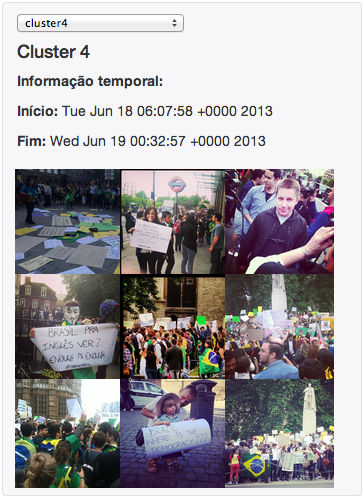
\includegraphics[width=0.9\linewidth]{./figures/olhopassarinho/c4_ex1_im33_e33_t33_1819}
	\caption{ Visualização de uma amostra de imagens do \textit{cluster} 4 }
	\label{subfig:im42}
	\end{subfigure}
\caption{Exemplo da visualização do conteúdo visual de dois \textit{clusters} calculados com 33.33\% do peso para cada uma das dimensões}
\label{fig:im40}
\end{figure}


\section{Sumário}

Em suma, neste capítulo foi apresentado a concretização da integração do modelo da representação da informação visual desenvolvido, descrito no Capítulo~\ref{chap:chap3}, para estender o TweeProfiles. 

O primeiro passo passou pelo cálculo as matrizes de distância para a dimensões temporal e espacial. Isto permitiu efetuar combinação entre as várias matrizes das diferentes dimensões. Em seguida foi efetuado o processo de \textit{data mining} que culminou nos diferentes \textit{clusters} para diferentes combinações. Feito isto, foi então desenvolvid a aplicação Web que permitiu a visualização dos resultados e controlo das diferentes combinações. Por fim foram apresentados alguns resultados ilustrativos.

Os exemplos escolhidos para apresentar os resultados ilustrativos pretenderam demonstrar as diferentes potencialidades da ferramenta, focando principalmente na atribuição de pesos às diferentes dimensões e na visualização dos resultados dessas mesmo combinações. Para além das combinações demonstradas, é possível realizar mais seis combinações diferentes. Existe também ainda a possibilidade de escolher um dos três diferentes intervalos de tempo que correspondem a cada um dos subconjuntos de dados previamente criados.


